\documentclass[conference,onecolumn]{IEEEtran}

\usepackage[nolist]{acronym}
\usepackage[backend=bibtex]{biblatex}
\usepackage{graphicx}
\usepackage{hyperref}
\usepackage{pdfpages}

\addbibresource{../master-thesis.bib}

\begin{document}

  \title{Proposal: Creating a web-based model transformation UI (with GLSP)}

  \author{\IEEEauthorblockN{Florian Weidner}
    \IEEEauthorblockA{Philipps-University Marburg, Germany\\
      Department of Mathematics and Computer Science, Software engineering group\\
      May 06, 2025\\
  }}

  \maketitle

  \IEEEpeerreviewmaketitle

  \section{Motivation and introduction}
  \label{sec:motivation}

  In software engineering, often \ac{mde} is used to increase development productivity and quality. Concepts are modeled closer to the domain, so that they describe important aspects of a solution with human-friendly abstractions. The models can also be used to generate application fragments, that can be directly used as source code. In the process of \ac{mde}, many activities need to transform source models into different target models, while following a set of transformation rules. This model transformation process is based on algebraic graph transformations. A metamodel is used to model the structure and rules of the concept. The resulting transformation language can provide automatic model creation, development and maintenance activities. \cite{transformations-modeldriven} One framework to use \ac{mde} is \ac{emf} by the Eclipse Foundation. It provides a basis for application development, using modeling and code generation facilities. Much frameworks build upon \ac{emf}, providing various \ac{mde} tools like code generators, graphical diagramming, model transformation or model validation. \cite{emf} One model transformation framework is Henshin. \cite{henshin-repo} It tries to provides model transformation capabilites with a high level of usability. \cite{henshin-usability} For metamodels it uses \ac{emf} Ecore files and for instance models \ac{emf} XMI files. The framework enables transformations on XMI instance files with a defined transformation language. It provides a graphical and textual syntax to create these transformation rules. \cite{henshin-repo} Henshin can be used as a eclipse plugin. Eclipse makes it easy to access, but especially for new users, the heavy editor makes the use of Henshin unintuitive.

  Therefore the goal exists to create a graphical option to use the Henshin model transformations without the overhead of the heavy eclipse editor. A web-based graphical editor would make the use of Henshin even more accessible and intuitive.

  \ac{glsp} is a open-source framework by the Eclipse Foundation to develop custom diagram editors for distributed web-applications. \cite{glsp-repo} It can be used in Eclipse Desktop IDE, Eclipse Theia, Visual Studio Code and embedded in any website. With these fuctionalities, \ac{glsp} fits to create an accessible, intuitive application to create and apply Henshin model transformations.

  \section{Project Requirements}
  \label{subsec:requirements}

  The following requirements are a list of the functional and non-functional requirements that i came up with. The client should be integrated as a Eclipse Theia client. Additional clients can be added in the future without overhead effort.

  Functional requirements:

  \begin{itemize}
  
    \item \ac{emf} XMI instance files should be displayed in a graphical editor
    \item Henshin rule files should be displayed in a graphical editor
    \item \ac{emf} Ecore metafiles should be displayed in a graphical editor
    \item The instance editor should display all rules that can be applied to the instance model.
    \item Parameters of the rules should be editable when applying a rule.
    \item After applying a rule, the instance model should be updated and displayed in the instance editor as a temporal file that can be used to apply multible rules. The initial instance model should not be changed.
    \item The instance editor should provide editing functionality for the instance model.
    \item The Henshin rule editor should provide editing functionality for the transformation rules.
    \item The Ecore editor should provide editing functionality for the Ecore metamodel.

  \end{itemize}

  Once all functional requirements are implemented, the application should fully support a basic model transformation workflow. Its functionality should be equivalent to using the Henshin plugin within the Eclipse editor. It should be possible, that additional Henshin functionalities like State Space analysis or confilct and dependency analysis can be added in the future.


  Non-functional requirements:

  \begin{itemize}
    \item The application should be web-based and accessible via a web browser.
    \item The application should be responsive and work on different screen sizes.
    \item The application should be user-friendly and intuitive to use.
    \item The application should be performant and handle large models efficiently.
\end{itemize}

  \section{Basic architecture}
  \label{subsec:architecture}

  \ac{glsp} uses a client-server architecture. For the backend, the framework supports integration with EMF models as the underlying source for the diagrams. That makes the integration of Henshin easier, because all files are based on \ac{emf}. The \textit{HenshinRessourceSet} can be loaded over the \ac{emf} integration of \ac{glsp} directly. For the XMI instance files, the Henshin rule files and the Ecore metamodel files, a mapping to the \ac{glsp} internal graphical model needs to be implemented. \cite{eclipseGLSP}
    
  \section{Implementation}
  \label{subsec:implementation}

  \section{Preliminary table of contents}

  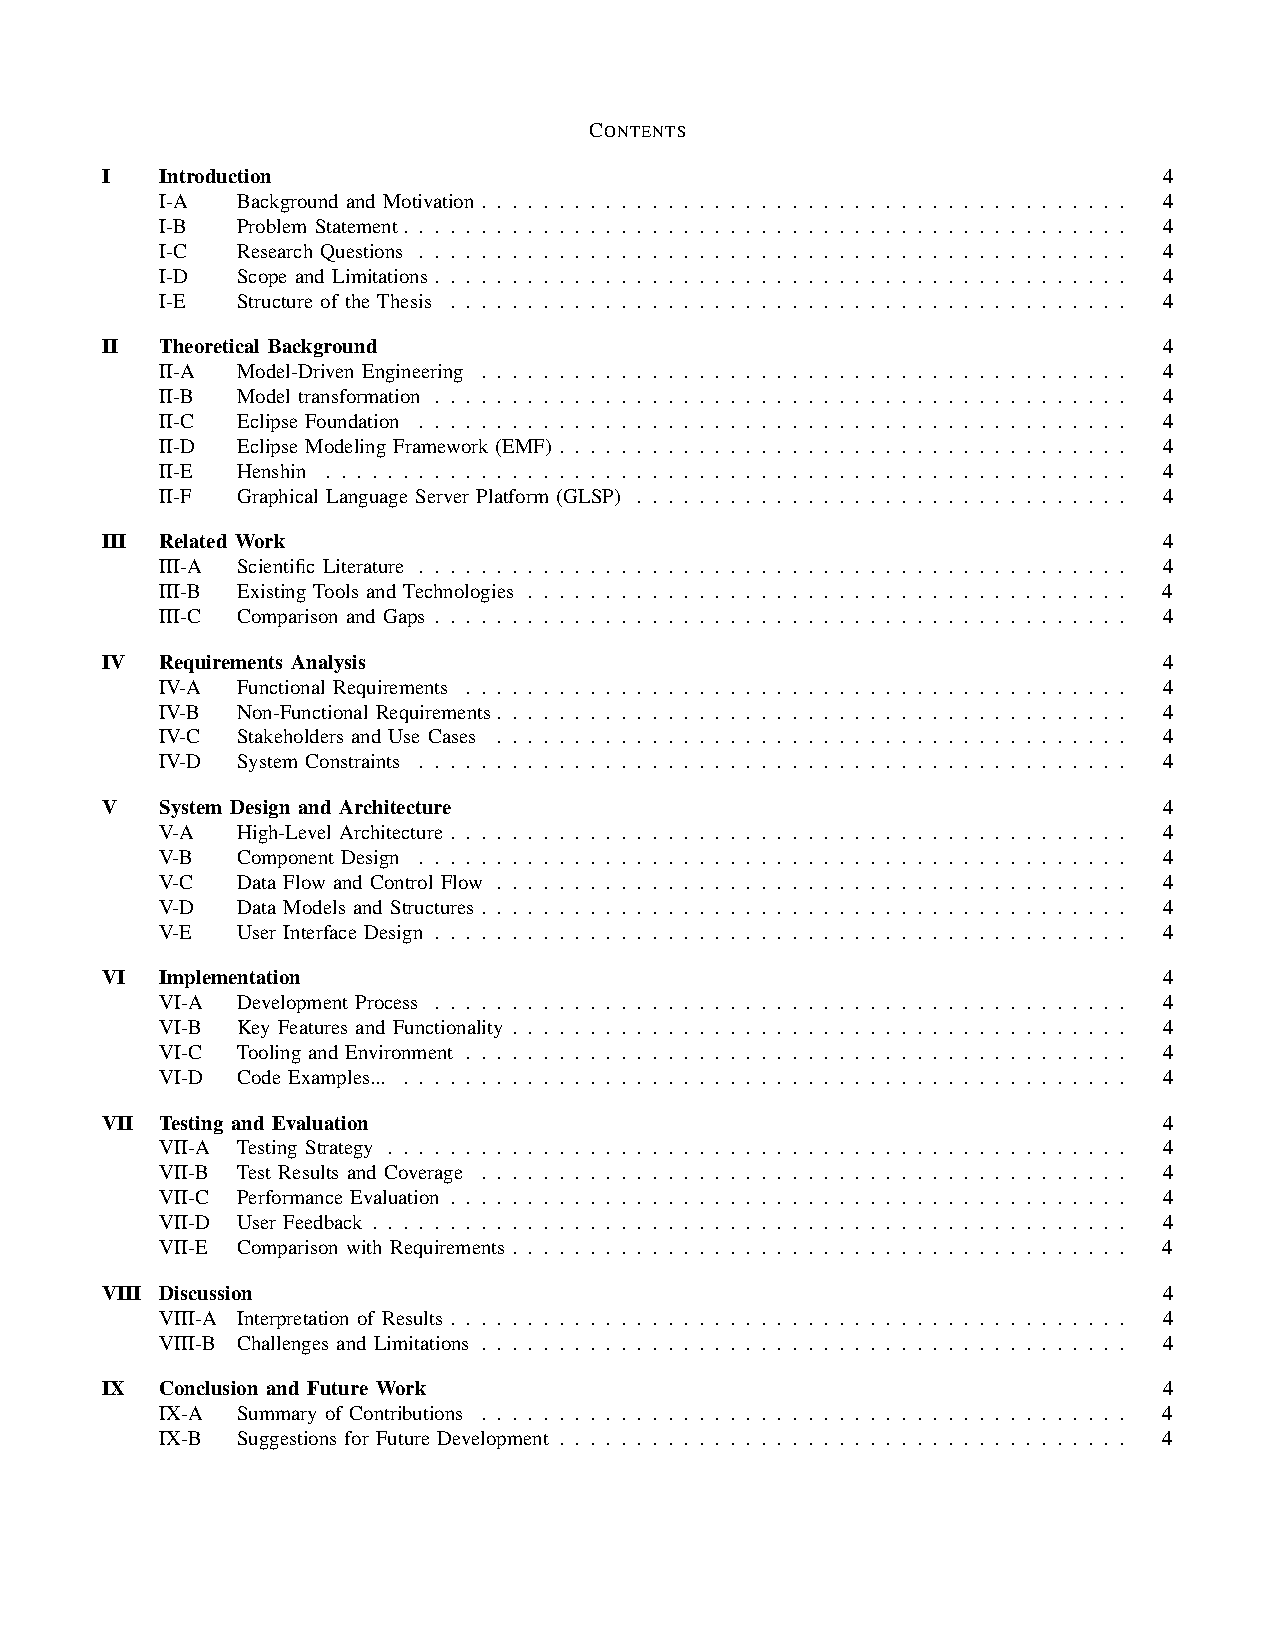
\includepdf[pages=1]{preliminary-toc.pdf}

  \section{Time schedule}
  The goal is to finish the project and the thesis at the end of August. From now on that includes 14 weeks. The three main tasks are the development of the application, writing the scientific work about the thesis and writing the final thesis.

  \begin{table}[h!]
    \centering
    \caption{Project development tasks}
    \begin{tabular}{|p{0.5cm}|p{8cm}|p{1cm}|p{1cm}|}
      \hline
      \textbf{Task No.} & \textbf{Description} & \textbf{Estimated Time Needed} & \textbf{Planned Completion} \\
      \hline
      1 & Creating a Prove of Concept to apply rules on an instance model & 2 weeks & 31. Mai \\
      2 & Design Frontend and System architecture & 1 week & 07. Juni \\
      

      \hline
    \end{tabular}
  \end{table}

  \begin{table}[h!]
    \centering
    \caption{Thesis writing tasks}
    \begin{tabular}{|p{0.5cm}|p{8cm}|p{1cm}|p{1cm}|}
      \hline
      \textbf{Task No.} & \textbf{Description} & \textbf{Estimated Time Needed} & \textbf{Planned Completion} \\
      \hline
      1 & basics chapter about model transformations & 1 week & 07.Juni \\
      1 & basics chapter about \ac{emf} and the Eclipse Foundation & 1 week & 07.Juni \\
      1 & basics chapter about Henshin and GLSP & 1 week & 07.Juni \\     

      \hline
    \end{tabular}
  \end{table}

  \section{Conclusion}


% 1 & Requirements analysis and specification & 1 week & Week 1 \\
%       2 & Design of system architecture & 1 week & Week 2 \\
%       3 & Implementation of EMF XMI instance viewer & 1 week & Week 3 \\
%       4 & Implementation of Henshin transformation rule viewer & 1 week & Week 4 \\
%       5 & Apply transformation rules to instance models & 1 week & Week 5 \\
%       6 & Editing functionality for transformation rules & 1 week & Week 6 \\
%       7 & Editing functionality for XMI instance models & 1 week & Week 7 \\
%       8 & Viewer and editor for Ecore metamodels & 1 week & Week 8 \\
%       9 & Integration and testing & 1 week & Week 9 \\
%       10 & Documentation and final review & 1 week & Week 10 \\

  \printbibliography

\begin{acronym}
  \acro{glsp}[GLSP]{Graphical Language Server Platform}
  \acro{emf}[EMF]{Eclipse Modeling Framework}
  \acro{mde}[MDE]{Model-Driven Engineering}
\end{acronym}

\end{document}
